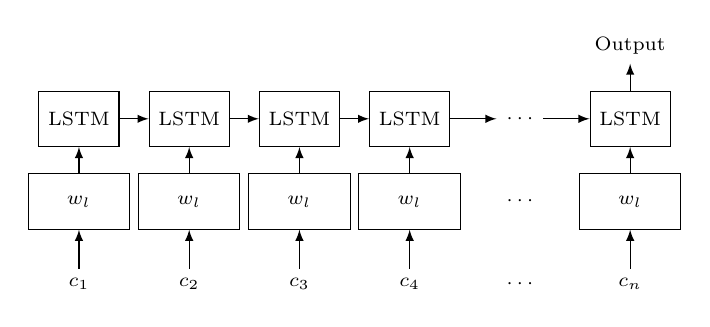
\begin{tikzpicture}[x=0.7cm, y=0.7cm, every node/.append style={text=black, font=\scriptsize}]
	\foreach \i/\l in {1/1, 2/2, 3/3, 4/4, 6/n}
	{
		\node[draw=black, minimum height=20] (1\i) at (2*\i, 0) {LSTM};
		\node[draw=black, minimum height=20, text width=30, align=center] (2\i) at (2*\i, -1.5) {$w_l$};
		\node[text width=30, align=center] (3\i) at (2*\i, -3) {$c_\l$};		
	}
	
	\node (15) at (2*5,0) {$\cdots$};
	\node (25) at (2*5,-1.5) {$\cdots$};
	\node (35) at (2*5,-3) {$\cdots$};	
	
	\foreach  \i/\j in {1/2, 2/3, 3/4, 4/5, 5/6}
	{
		\draw [-latex] (1\i) -- (1\j);
	}
	
	\foreach  \i in {1,2,3,4,6}
	{
		\draw [-latex] (2\i) -- (1\i);
		\draw [-latex] (3\i) -- (2\i);
	}	
	
	\draw[-latex] (16) -- +(0,1) node [anchor=south] {Output};
	

\end{tikzpicture} 